\chapter{Event reconstruction and simulation}
\label{chap:reconstruction}

After the results of proton collisions have been observed in the
various subdetectors that comprise \CMS, the physical objects produced
in each collision event are reconstructed. Through this
reconstruction,
an overall analysis of the underlying physical process can be carried
out. To aid in classifying the types of collision events, \MC
simulations are also carried out. The reconstruction algorithms and
simulations that are relevant to the search for supersymmetry
presented in this thesis are described in this chapter.

\section{Tracks and vertices}
\label{sec:tracks_reco}

As charged particles pass through the \CMS tracker they leave energy
deposits, known as \emph{hits}, in each layer. These hits are
reconstructed as tracks with the \ac{CTF} algorithm
\cite{Chatrchyan:2014fea}, which tries to associate hits that belong
to a single charged particle. This allows for the determination of the
path taken by the charged particle, its \emph{track}. The curvature of
the particle as it passes through the magnetic field is then used to
determine its momentum. The steps of the algorithm are as follows:

\begin{itemize}
\item{Initially two or three hits in the inner layers of the tracker
are taken as seeds for initial track candidates. Quality
criteria are applied on the selected hits, which retain only promising
seeds.} 
\item{Each seed is extrapolated along the expected trajectory using a
Kalman filter \cite{Fruhwirth:1987fm} with a helical tracking
hypothesis. This allows the seeds to be associated with hits in an
outer tracker layer while taking account of uncertainties in the
measurement.} 
\item{The extrapolation is carried out recursively into the subsequent
tracker layers until the outer-most layer is reached.} 
\item{Once the tracking candidates are found, additional quality
criteria are required to reject fake tracks.}
\item{This series of steps is repeated up to six times and the hits
associated with identified tracks are removed after each iteration. }
\end{itemize}

Track reconstruction efficiencies for a variety of charged particles
are shown in Fig.~\ref{fig:tracks_reco} as a function of \pt and
$\eta$. In the central region of the detector all particles with a \pt
from 10 to 100~\gev are reconstructed with a 90-100\% efficiency. In the
forward detector region this efficiency remains above $\sim80\%$.
%fake rate? leave out for now...

\begin{figure}
\begin{center}
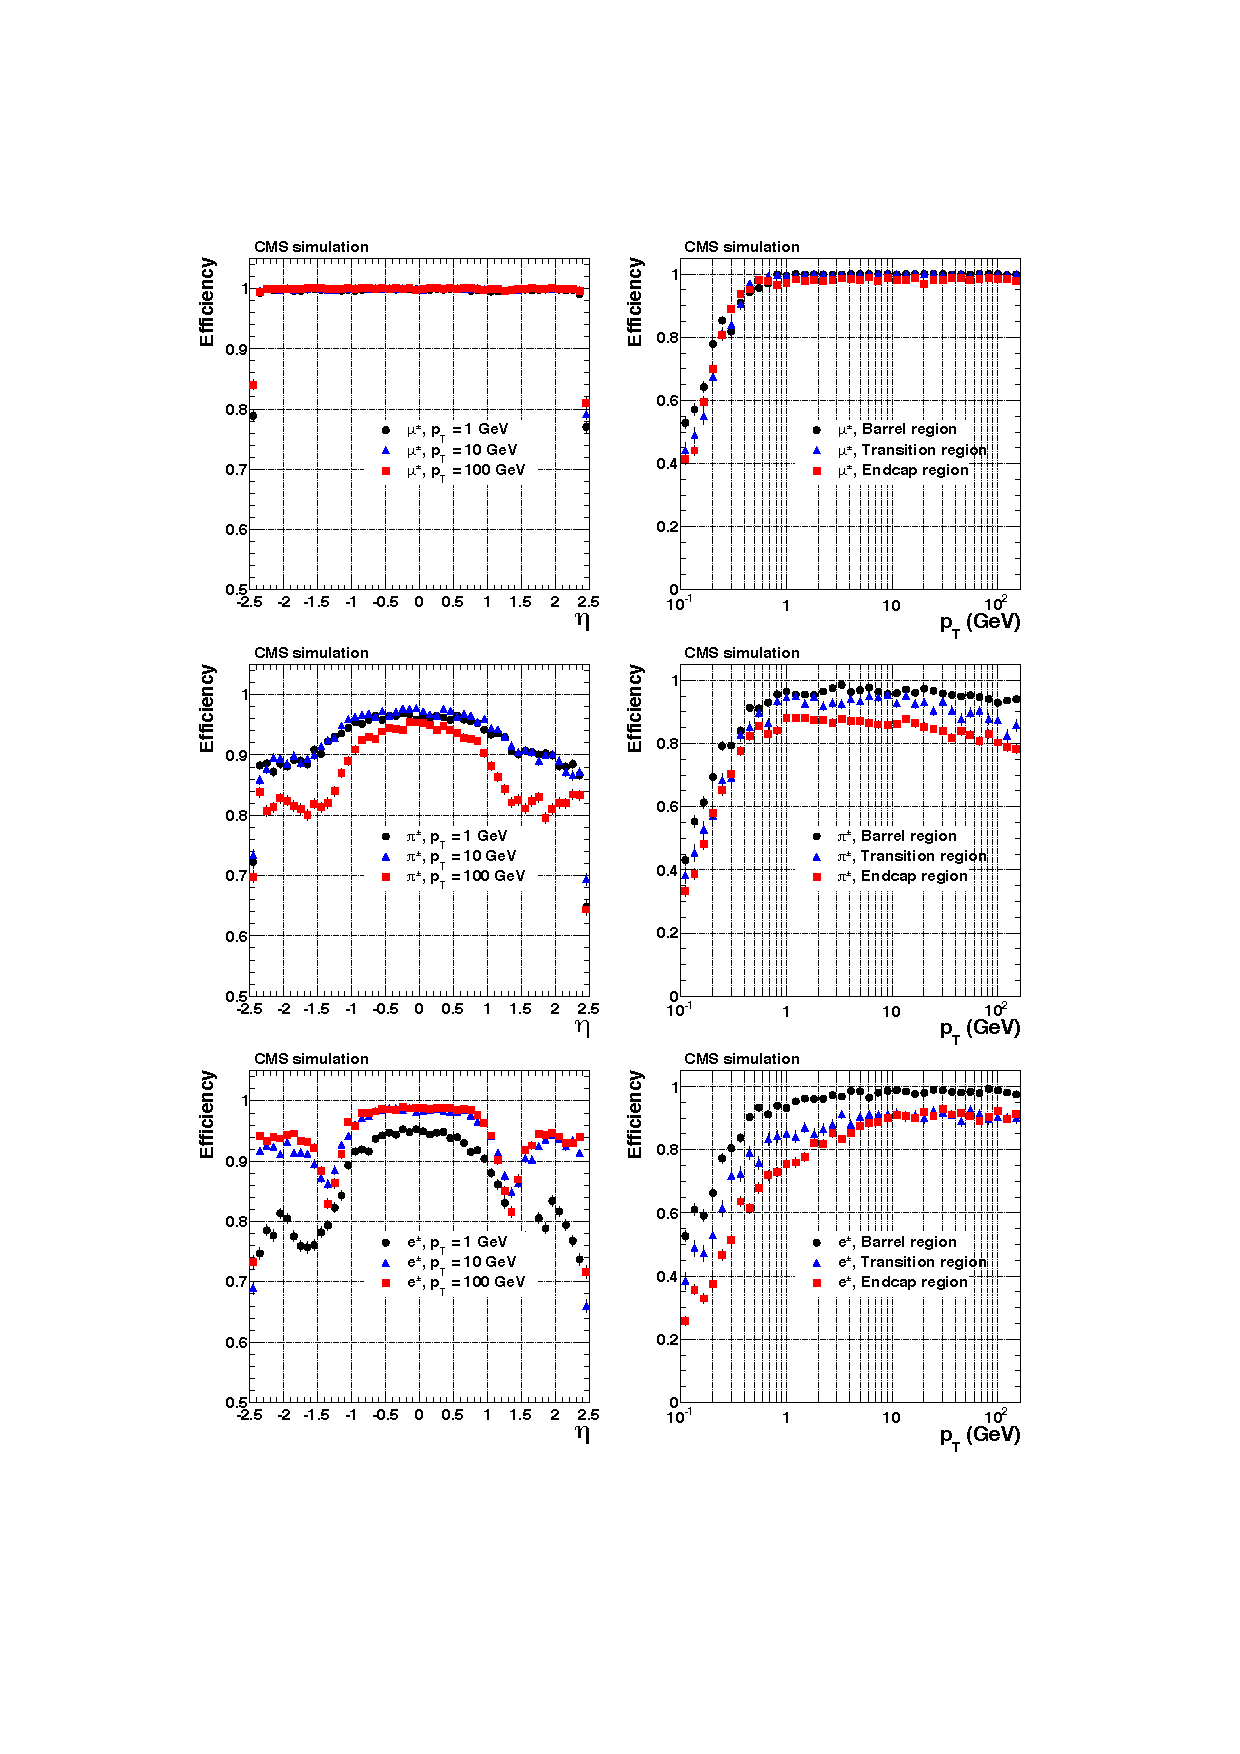
\includegraphics[width=0.8\linewidth]{figs/reconstruction/trackerPerformance} \end{center}
\caption{Efficiencies of track reconstruction for different charged
particles as a function of \pt and $\eta$. Muons are shown at the top,
pions in the middle and electrons at the bottom. The barrel,
transition and endcap regions are defined by the $\eta$ intervals of
0-0.9, 0.9-1.4 and 1.4-2.5 respectively.  For all the tracks
\emph{high-purity} quality requirements are made
\cite{Chatrchyan:2014fea}}
\label{fig:tracks_reco} \end{figure}

After charged particle tracks are reconstructed, they can be used to
infer the positions of the different proton-proton collisions in the
event, known as interaction vertices. Tracks are required to originate
from a region that is compatible with the \LHC \emph{beamspot}, the area
in which the proton beams cross and collisions occur. The
$z$-coordinates of tracks at the closest point of approach to the
beamspot are taken as an input for the deterministic annealing
clustering algorithm \cite{726788:DA}. This finds the most probable
vertex positions and assigns each track to a vertex. The final
$x$,$y$,$z$ position of these vertices is then found using the
adaptive vertex fitter \cite{Waltenberger:2008zz}. This assigns the
most probable position of the vertex for the given set of input
tracks. Quality criteria are then applied to reject fake vertices,
they are chosen in such a way as to remain efficient for real vertices
that typically have a large number of tracks compatible with them.
Finally, the \emph{\ac{PV}} is determined as the vertex with
tracks that have the greatest scalar sum of \pt. Other vertices are
then initially attributed to \PU.  However, vertices that are
displaced from the initial proton collision are common signatures of
unstable particles that decay within the detector, such as
$b$-hadrons. These can be found in subsequent levels of
reconstruction.

The efficiency for finding the \ac{PV} as a function of the
number of tracks in a cluster can be seen in
Fig.~\ref{fig:vertex_reco}. The efficiency increases to close to
$>99\%$ for events with $\ge 3$ tracks. The vertex resolution reaches
$\sim10~\mu$m in $x,y$ and $\sim15~\mu$m in $z$ with $>40$
reconstructed tracks.

\begin{figure}
\begin{center}
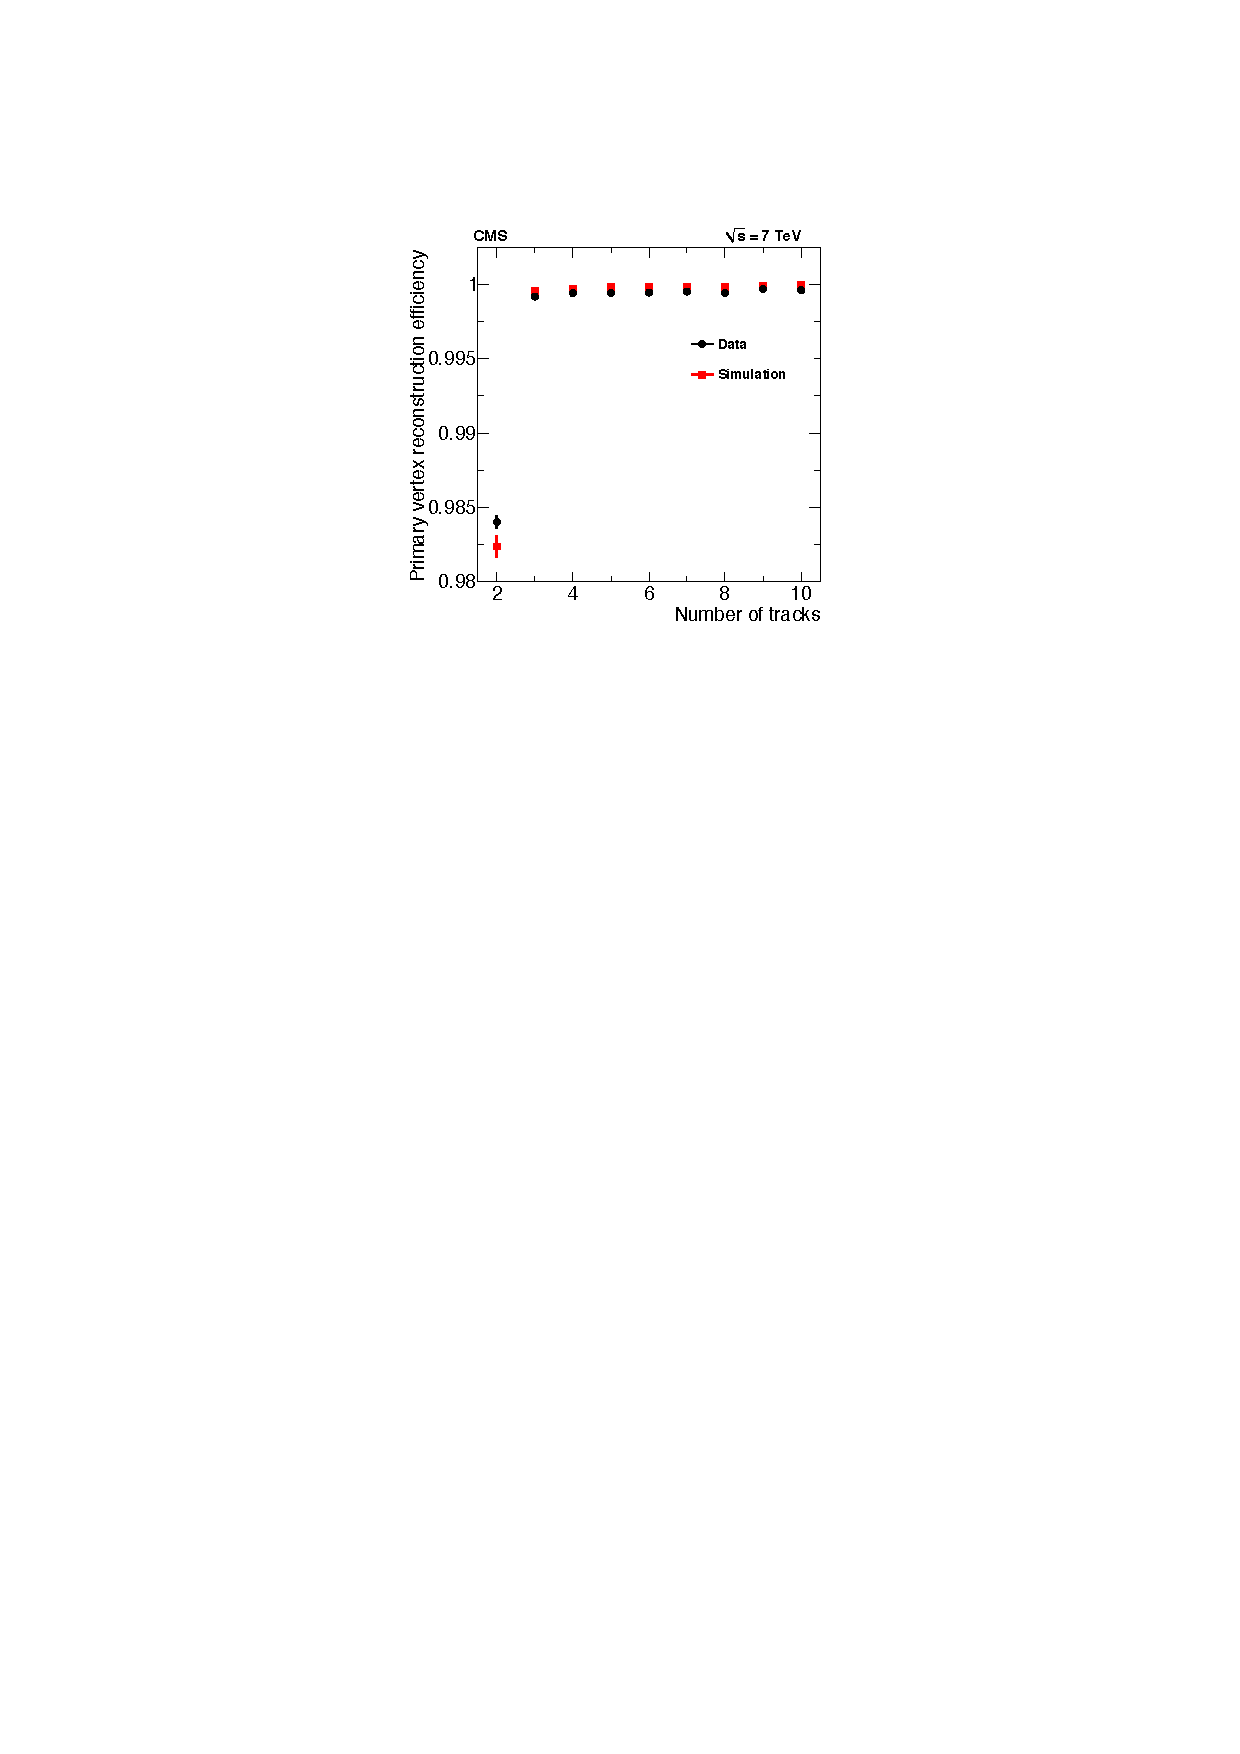
\includegraphics[width=0.5\linewidth]{figs/reconstruction/vertexPerformance} \end{center}
\caption{ The vertex reconstruction efficiency as a function of the
number of tracks originating from the vertex. Measured in data and
simulation for $\sqrt{s}=7~\tev$ proton collisions.
\cite{Chatrchyan:2014fea}}
\label{fig:vertex_reco} \end{figure}


\section{Particle flow}
\label{sec:pflow_reco}

Each of the subdetectors of \CMS provide complimentary information
about the different types of particles that pass through the detector.
This is exploited to identify the different types of particle with the
\PF algorithm
\cite{CMS-PAS-PFT-09-001,CMS-PAS-PFT-10-001,CMS-PAS-PFT-10-002}. As
\CMS has accurate momentum resolution in the tracker and a high
granularity \ECAL this algorithm allows both to augment the
measurement of objects in the \HCAL. This then allows calibrations
that are specific to both charged and neutral hadrons to be applied. 

The \PF algorithm searches for a set of individual particles that are
known as \PF \emph{candidates}. They are then classified as charged or
neutral hadrons, photons, muons or electrons. The set of \PF
candidates can then be utilised to calculate other event level
variables, such as for jet reconstruction described in
Sec.~\ref{sec:jets_reco}.
%Do i need to describe how clusters are made more?

The algorithm starts by taking the tracks, which are reconstructed as
in Sec.~\ref{sec:tracks_reco}, along with clusters of energy
in the calorimeters, which are reconstructed separately in the \ECAL and
\HCAL. Clusters are paired with tracks if the track trajectory is
compatible with the cluster position. These pairs are then used to
identify charged particles. Electrons and hadrons are typically
differentiated based on the proportion of energy they deposit in the
\ECAL or \HCAL. Electrons will deposit nearly all their energy in the
\ECAL whereas hadrons will deposit much more in the \HCAL. A similar
pairing between tracks and hits in the muon system is used to identify
muons. 

Neutral particles are then identified through calorimeter clusters
that do not have a compatible track associated to them. Photons, for
example, will leave a significant \ECAL deposit with no track, which
would be present for electrons. Similarly, neutral hadrons will leave
significant deposits in the \HCAL with no associated track.

\section{Electrons and photons}
\label{sec:electrons_reco}

Electrons and photons interact with the \ECAL in a similar way.
The reconstruction techniques used for both are therefore very similar, with
the main difference being the lack of a track in photon reconstruction.
As electrons interact with the tracker, they lose on average $33\%$ of
their energy before reaching the \ECAL \cite{1748-0221-10-06-P06005}.
Most of this energy loss occurs through bremsstrahlung, which has a
non-Gaussian loss distribution. As the Kalman filter that is used in
track reconstruction assumes Gaussian energy losses, another specialist
track reconstruction for electrons is employed, known as the Gaussian
Sum Filter algorithm \cite{Adam:815410}. To maintain a good energy
resolution, the photons that are produced during bremsstrahlung must
also be properly associated with the electron when clustering in the
calorimeter. As the electrons bend in the magnetic field but the
photons they emit do not, the calorimeter clusters are allowed to
extend along the azimuthal direction. These rectangular \ECAL windows
are know as \emph{superclusters}.

To form the superclusters in the barrel the \emph{hybrid} clustering
algorithm is used. A single seed crystal with a local maximum
transverse energy $E_T>1~\gev$ is identified and a rectangular
configuration of $3\times 1$ or $5\times 1$ crystals in $\eta$-$\phi$
is formed around it. The algorithm then looks in the $\phi$ region
adjacent to this rectangle up to $\Delta\phi\pm 0.3$.
Additional rectangular regions that have $E_T>100$~MeV are kept and
grouped to form the supercluster. In the endcaps the \emph{multi $5\times
5$} algorithm is used instead, which aggregates $5\times 5$ arrays of
crystals within $\Delta\eta<0.07$ and $\Delta\phi<0.3$ of the seed.

Electrons are identified through a supercluster matched to a track, or
photons are identified through an unmatched supercluster. After
this, additional selection criteria are applied to suppress
backgrounds. The major backgrounds come from misreconstructed hadronic
jets or semi-leptonic decays of heavy quarks. To suppress these
backgrounds, cuts
are made on the ratio of energy deposits in the \HCAL and the \ECAL, the
difference in direction between the track and supercluster (in the
case of electrons) and the width of the cluster, which is larger for
hadrons.

\section{Muons}
\label{sec:muons_reco}

Unlike electrons and photons, muons are minimally ionising so do not
lose much of their energy to the tracker or calorimeters
\cite{Chatrchyan:2008aa}. Muon reconstruction therefore
uses a combination of tracks and hits in the muon system. To maintain
high efficiencies across a wide range of muon energies, two algorithms are
utilised \cite{1748-0221-7-10-P10002}. The \emph{global} muon algorithm
functions in the same way as the \PF algorithm, mentioned in
Sec.~\ref{sec:pflow_reco}. To maintain efficiency for low energy muons
that have a lower probability of traversing the entire muon system
the \emph{tracker} muon algorithm is additionally used.

The global muon algorithm starts with hits in each layer of the muon
system that give an initial estimate of the position, energy and
direction of candidate muons. It then searches for tracks in the inner
detector that are compatible with this candidate. If this is the case,
the track is extrapolated to the hits in the muon system using a
Kalman filter, similar to the way tracks are reconstructed in
Sec.~\ref{sec:tracks_reco}. 

The tracker muon algorithm starts with tracks with $\pt>0.5~\gev$ and
extrapolates them into the muon system, again with a Kalman filter. If
any of these tracks can be matched to at least one muon chamber hit it
is considered to be a muon. For muons with $\pT<200~\gev$ the tracker
provides the highest resolution energy measurement, while the muon
system provides a better resolution for the straighter, higher \pT,
tracks.

To reduce the background from hadrons that have punched through the
\HCAL or muons that do not originate from the primary vertex, such as
those from cosmic
rays, a series of selections are applied to the reconstructed
muon candidates. These include a quality requirement on the fit of the
tracks, a minimum number of hits in the muon systems and a track
compatible with originating from the beamspot. A different set of
criteria can be applied to trade off the efficiency and fake rate of
the muons. After the application of a \emph{tight} set of criteria, the
efficiency of muons with $\pT>10~\gev$ is measured to be $>96\%$,
shown in Fig.~\ref{fig:muonEff}.

\begin{figure}
\begin{center}
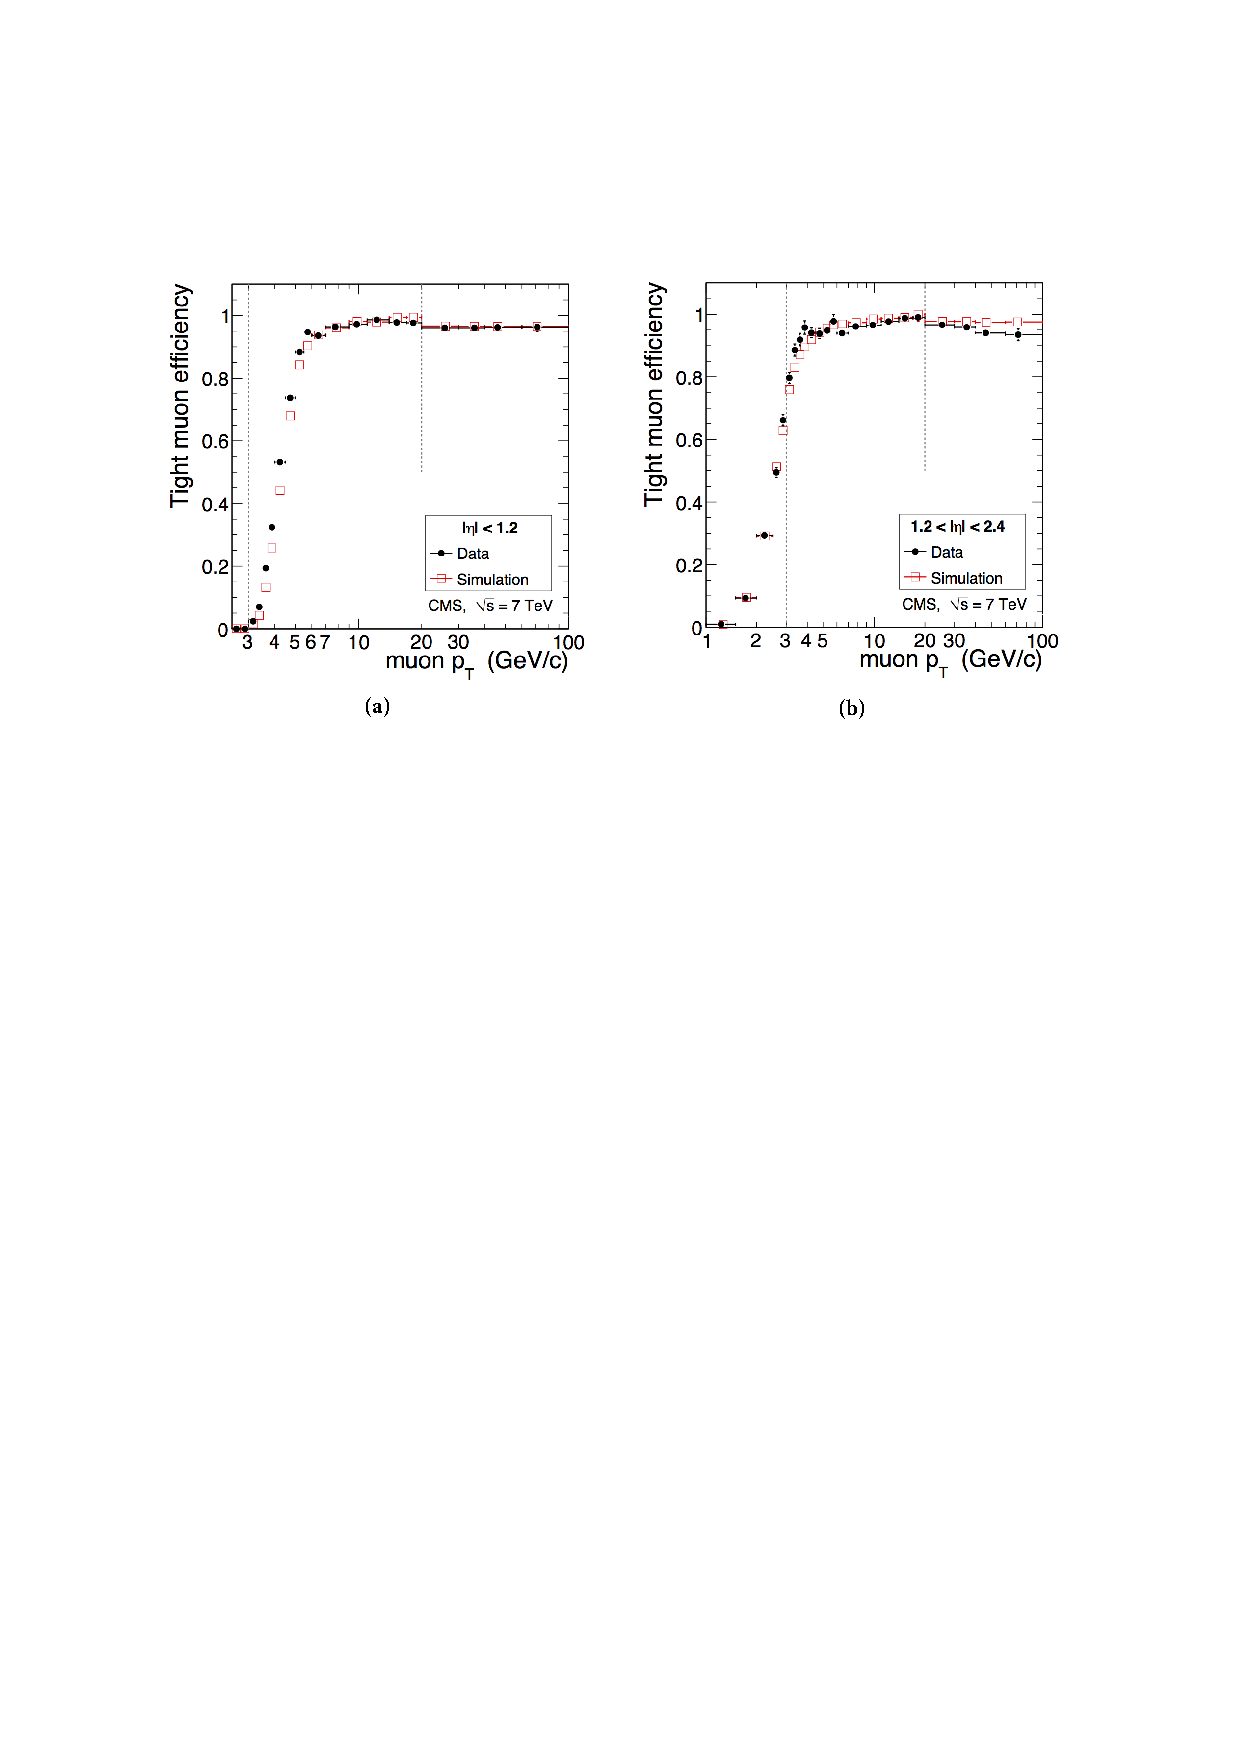
\includegraphics[width=0.9\linewidth]{figs/reconstruction/muonEff} \end{center}
\caption{ The tight muon reconstruction efficiency as a function of the
\pt of the muon in $\sqrt{s}=7~\tev$ proton collisions. The efficiency
is measured separately in the barrel (a) and endcap (b) regions.
\cite{1748-0221-7-10-P10002}}
\label{fig:muonEff} \end{figure}

\section{Jets}
\label{sec:jets_reco}

As there is a very high probability that proton collisions will
produce quarks and gluons, identifying and measuring them is a crucial part of
object reconstruction in \CMS. This is particularly relevant when
searching for strongly produced \SUSY particles as they typically
decay via hadrons to the \LSP, as described in
Chapter~\ref{chap:theory}. Due to the nature of the strong force,
high $\pT$ quarks and gluons undergo immediate hadronisation. The
result of this is a collimated shower of, predominantly hadronic,
particles. To reconstruct the quarks and gluons produced in
an event these collimated showers of particles are clustered and
reconstructed as \emph{jets} \cite{Salam2010}.

\subsection{The anti-$k_T$ clustering algorithm}

When determining the clustering algorithm to be used, the theoretical
behaviour of hadronisation must be taken into account
\cite{Salam2010}. Specifically, jets can undergo soft gluon radiation
of arbitrarily low energy gluons with a high probability.
Similarly, a gluon can split into two, almost collinear, gluons that share its energy.
The final result of the clustering algorithm cannot not depend
on either of these things happening. It must be both
\emph{infrared safe} and \emph{collinear safe}. The jet algorithms used in \CMS are
typically some form of a \emph{sequential recombination algorithm} that
fulfills the above criteria. After defining a \emph{distance}
between all pairs of particles in the event, $d_{ij}$, and a distance
from each particle to the beamline, $d_{iB}$, the algorithm undertakes
the following steps:
\begin{itemize}
\item{Calculate $d_{ij}$ for all pairs of particles in the event and
$d_{iB}$ for each particle.}
\item{If a value of $d_{ij}$ is smallest, combine the pair of particles
with this distance into a single new particle and start again.}
\item{If a value of $d_{iB}$ is smallest remove this particle from the
list of particles, classify it as a cluster and start again.}
\item{Stop when there are no more particles remaining.}
\end{itemize}
For the sequential recombination algorithms used by \CMS the distance
parameters used are defined as:
\begin{equation} \label{eq:antiktdij}
d_{ij} = \textrm{min}(p_{Ti}^{2k},p_{Tj}^{2k})\frac{\Delta R_{ij}^2}{R^2} ,~~~~d_{iB} = p_{Ti}^{2k}
\end{equation} 
for particles $i$ and $j$ where $k=-1,0,1$, $\Delta R$
is the separation in the $\eta$-$\phi$ plane and $R$ is a fixed
parameter that sets the jet size. The most commonly used of the \CMS
algorithms has $k=-1$ and is known as the \emph{anti-$k_T$} algorithm
\cite{1126-6708-2008-04-063}. The anti-$k_T$ algorithm tends to
cluster circular jets built around the hardest particles in a
particular event. An area of $R=0.4$ is often
chosen as it contains the hadronic showers of most quarks and gluons
produced in $13-14~\tev$ proton collisions, while remaining
insensitive to contamination from \PU.

\subsection{Jet identification}

For the results presented in this thesis the \textsc{FastJet}
\cite{Cacciari2012} package is used to cluster the \PF candidates,
that are described in Sec.~\ref{sec:pflow_reco}. The
anti-$k_T$ algorithm is used with $R=0.4$. The \PF candidates
add information from the tracker when
calculating the momentum contribution to each jet from charged
particles. As jets typically consist of 65\% charged hadrons, 25\%
photons and 10\% neutral hadrons, this gives a significant improvement over
clustering the calorimeter deposits on their own. 

To reject fake jets from background sources or detector noise,
additional selection is applied to jet candidates. The \emph{loose} set of
criteria for jets provides an 84\% suppression of fake jets while
maintaining a $>99\%$ efficiency for real jets. It requires at least
two \PF candidates; $<99\%$ of the jet to come from only hadrons,
photons or electrons; and at least one charged track.

\subsection{Jet energy corrections}
\label{sec:reco_jec}

Due to the imperfect resolution of the \CMS detector, the initial
measured transverse momentum, $p_T^{raw}$, of a jet does not
necessarily match the energy of the particle that initiated the jet.
The difference between the \emph{raw} \pT and the \emph{true} \pT typically
depends on the \pT of the jet and its position in the detector, along
with components of the jet that are measured by different
subdetectors. To correct the raw \pT of the jet, a correction is
applied with the functional form
\cite{1748-0221-6-11-P11002}:
\begin{equation}
p_T^{cor}=C^{Off}(p_T^{raw},\rho,A_j)\cdot C^{Rel}(\eta)\cdot
C^{Abs}(p_T^{Rel})\cdot C^{Res}(p_T^{Abs})\cdot p_T^{raw}.
\end{equation}

The first step is the offset calibration, $C^{Off}$, which performs a correction
that removes the effect of other jets originating from \PU in the jet
cone. Initially, the contribution made by charged particles that do
not originate from the primary vertex is removed. This process is
known as \ac{CHS}. The remaining contribution from neutral \PU
particles is corrected using jet area subtraction
\cite{Cacciari:2007fd}. In this case the jet area, $A_j$ is multiplied
by the average pileup energy density, \rho. The value of \rho is
determined from the energy density of \PF candidates across the entire
detector.  Next, a relative correction, $C^{Rel}$, is applied as a
function of the \eta of the jet. This compensates for the differing
response of different parts of the detector across different
pseudorapidity ranges. An absolute correction, $C^{Abs}$ is then
applied on the output of the first two calibration steps, $p_T^{Rel}$.
This correction is designed to correct the dependence of the jet \pT
on the magnitude of the measured \pT. These two corrections are
calculated using information taken from both simulation and data. %Zbalance and dijet balance.
The final correction, $C^{Res}$, is applied only to data and not
simulation. This is designed to correct the residual differences in
the \pT and $\eta$ response between the data and simulation. The
magnitude of the corrections as a function of $\eta$ for two
representative values of \pT can be seen on Fig.~\ref{fig:jec}.

%put in performance figure?

\begin{figure}
\begin{center}
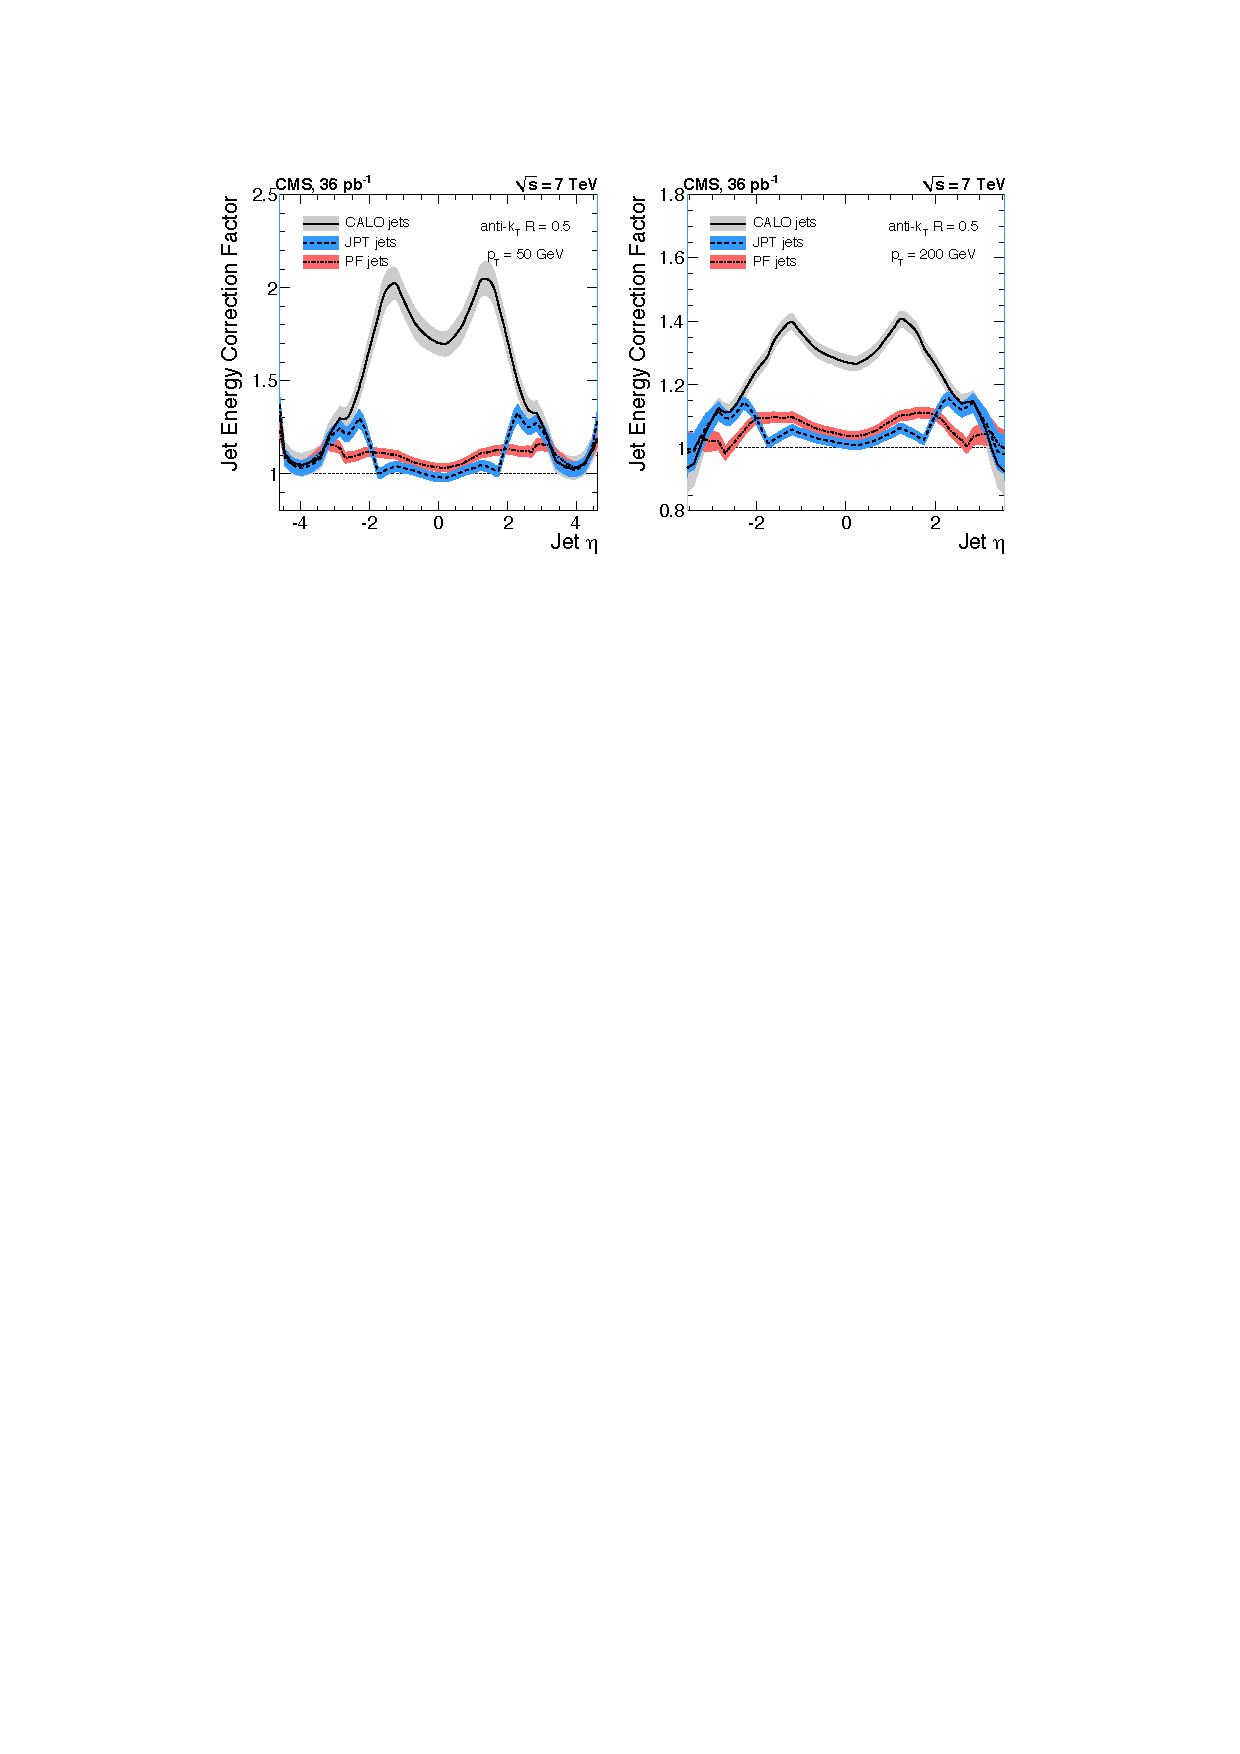
\includegraphics[width=0.9\linewidth]{figs/reconstruction/jec} \end{center}
\caption{The jet energy correction factors and their corresponding
uncertainty as a function of jet \eta
for jets with $\pT=50~\gev$ (left) and jets with $\pT=200~\gev$
(right) for different types of jet reconstruction. The correction for jets
reconstructed with \PF candidates is shown in the red line, the CALO
label indicates jets reconstructed purely with calorimeter deposits
and no tracker information \cite{1748-0221-6-11-P11002}}
\label{fig:jec} \end{figure}

\subsection{Tagging $b$-jets}
\label{sec:reco_btag}

The $b$-quark is of particular interest when searching for
indications of new physics. The production of these
quarks is relatively rare in \SM interactions and often
indicate the presence of a top quark that has decayed to a
$b$. In a wide range of \SUSY models the decay via top quarks is
favoured over other, lighter quarks. It is therefore very advantageous
to have a way of identifying jets as originating from $b$-quarks,
known as \emph{$b$-tagging}.

As $b$-hadrons have a relatively long lifetime, $\tau\sim 1.5$~ps
\cite{PhysRevD.86.010001}, they typically travel $c\tau\sim 450~\mu$m
from the primary vertex before decaying. The \CMS tracker has a
spatial resolution of $\sim 30~\mu$m for $\sim 5~\gev$ tracks
\cite{Chatrchyan:2008aa}, which means the displaced vertex created by
the $\sim 5~\gev$ mass $b$-quarks can be resolved. This is exploited
by the \ac{CSVv2} algorithm used for $b$-tagging in Run~2
\cite{CMS-PAS-BTV-15-001}. This algorithm uses a neural net with
detector inputs, including vertices identified by the tracker that are
displaced from the primary vertex and associated to the jet and
information about the tracks originating from this vertex.

As with the other physics object definitions in this chapter,
different selection criteria can be chosen to trade-off the mistag
rate and efficiencies for $b$-tagging. For each working point a
different discrete cut on
the \ac{CSVv2} discriminator is chosen, its distribution is shown in
Fig.~\ref{fig:bTag}. A \emph{medium} working point cut of 0.8 corresponds to
a tagging efficiency of $\sim 69\%$ and a mistag rate of $\sim 1\%$
\cite{CMS-PAS-BTV-15-001}. 

\begin{figure}
\begin{center}
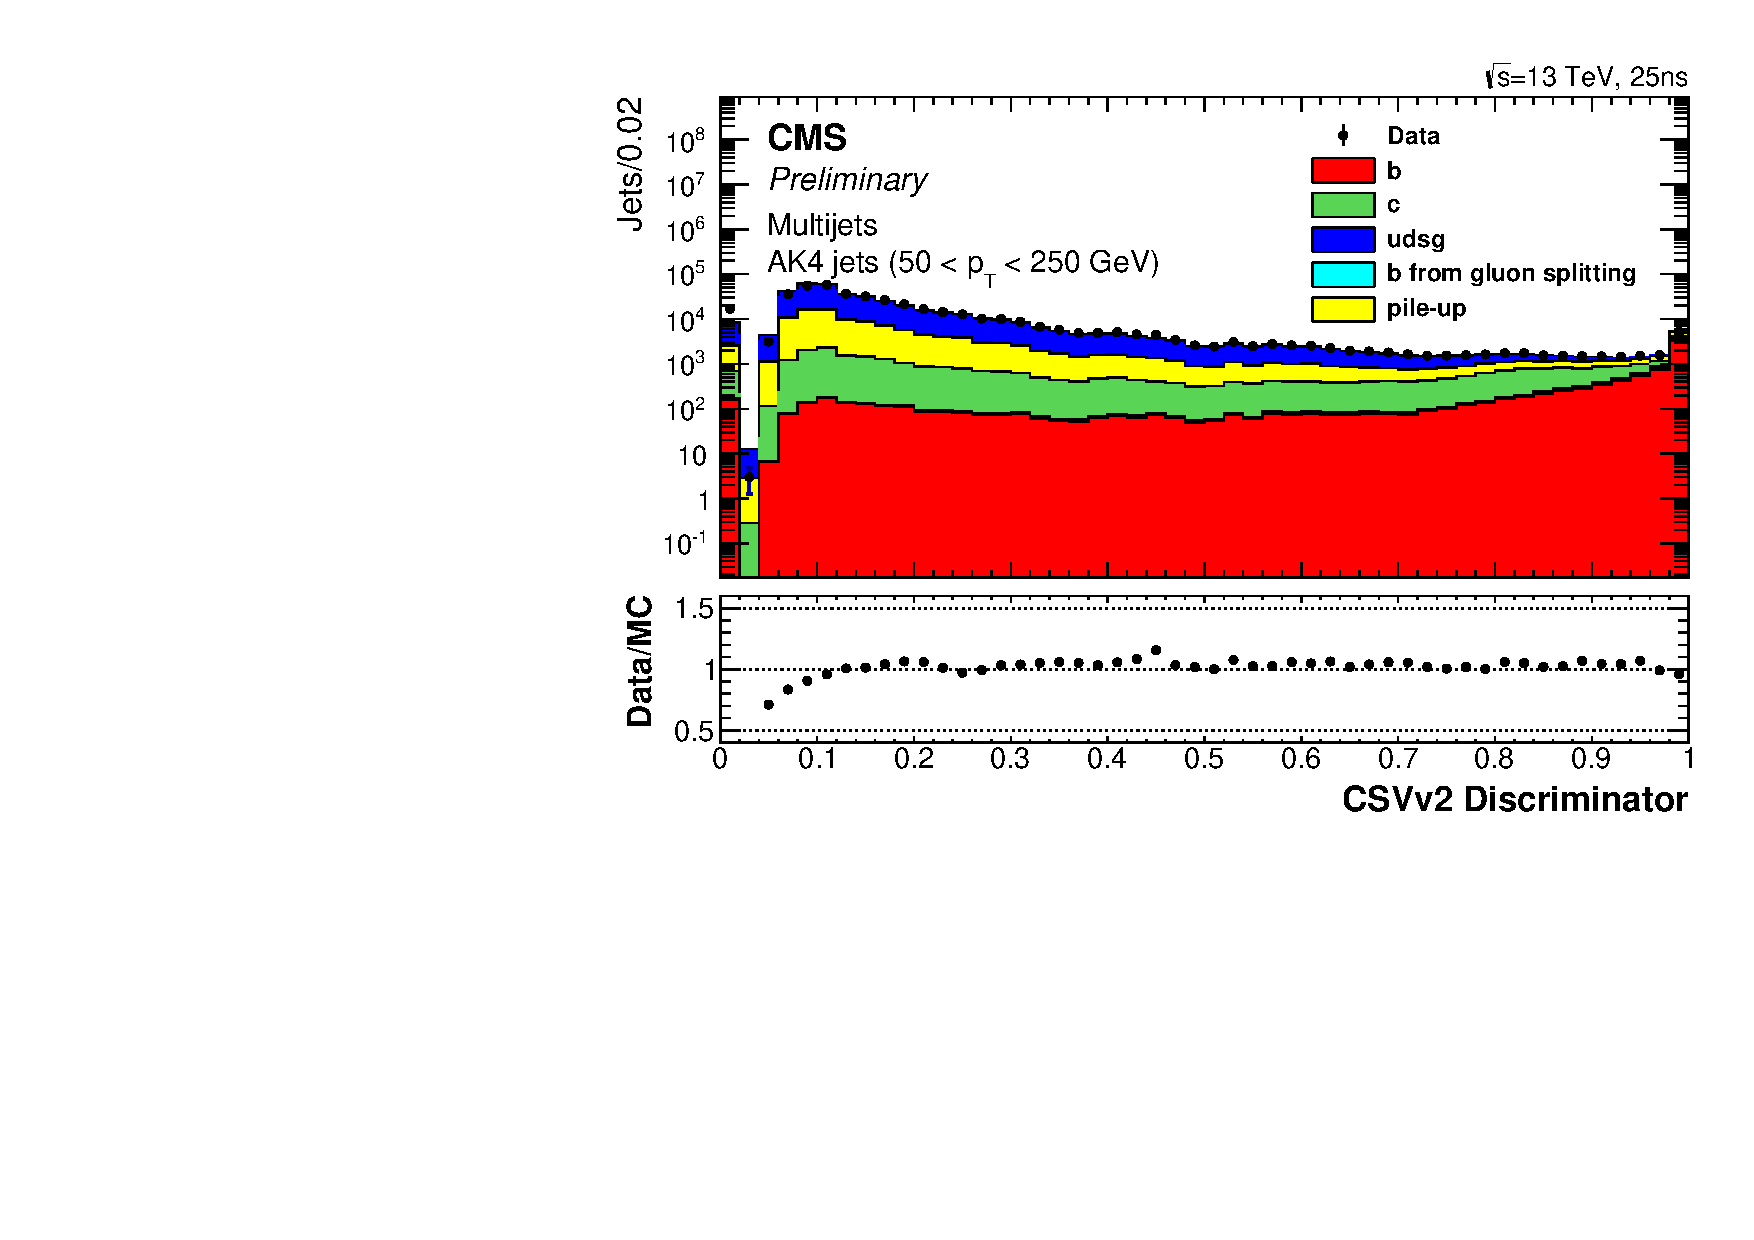
\includegraphics[width=0.7\linewidth]{figs/reconstruction/bTag} \end{center}
\caption{ The distribution of the discriminator \ac{CSVv2} algorithm
for $b$-tagging in multijet events. Tagged jets are clustered with the
anti-$k_T$ algorithm with $R=0.4$ and span $50<\pT<250~\gev$. A
working point is chosen to trade off b-tagging efficiency for mistag
rate by making a cut on the discriminator \cite{CMS-PAS-BTV-15-001}.}
\label{fig:bTag} \end{figure}

\section{Isolation and jet cross-cleaning}
\label{sec:reco_iso}

It is often important to differentiate \emph{prompt} leptons produced
directly in the primary vertex from those that are the result of decays
of other particles, such as those in hadronic jets. To do this an
\emph{isolation} variable, $I^{\textrm{rel}}$, is defined for each
lepton. To construct it the \pT of the \PF candidates within a cone
around the lepton are summed and the estimated neutral-charged
contribution of \PU within that cone is subtracted. This is then
divided by the \pT of the lepton in question, $\pT^l$. In the case
that the lepton is part of a jet $I^{\textrm{rel}}$ will have a large
value, this will not typically be the case if it is prompt.

In the work presented in this thesis, two variants of cone size are
used. In the standard case, denoted $I^{\textrm{rel}}$, a cone size
of $\Delta R=0.3$ is used. To maintain acceptance to leptons produced
in the decays of boosted objects, such as top-quarks, a
\emph{mini-isolation} can be defined that has a variable cone that
depends on the \pT of the object. A value of $\Delta R=0.2$ is chosen
for $\pT^l<50~\gev$, but this is scaled down to a minimum $\Delta
R=0.05$ for $\pT^l>200~\gev$.

The contribution from \PU is typically estimated in two different
ways. For \emph{effective-area} correction the average \PU energy
density of neutral particles, $\rho^{\textrm{neutral}}$, is multiplied
by the area of the isolation cone, similar to the \PU correction
carried out in jets as described in Sec.~\ref{sec:reco_jec}. For the
\emph{$\Delta\beta$} correction, the energy of neutral particles is
estimated as half the energy from charged particles that originate
from \PU vertices in the cone. This ratio of charged to neutral
particles is determined from simulation. % reference??

To avoid isolated leptons being classified as jets, a
\emph{cross-cleaning} can be performed on the result of the jet clustering.
In this case, all jets that are within $\Delta R=0.4$ of an isolated
lepton are removed from the event.

\section{Missing transverse energy (\met) and energy sums}
\label{sec:met_reco}

Weakly interacting particles, such as neutrinos or neutralinos, will
pass through all components of the \CMS detector. Their production can
therefore only be inferred from the imbalance of momentum in the decay
products of a proton collision that can be observed by \CMS. To
measure the magnitude and direction of the missing momentum the
missing transverse energy variable, \met, is defined as the negative
vector sum of the momentum, $\vec{p}_T$, of all the particles in an
event:
\begin{equation}
\met = -\sum{\vec{p}_T}.
\end{equation}
This is reconstructed taking the \PF candidates up to $|\eta|<5$ as
input \cite{1748-0221-10-02-P02006}. 

A correction is applied to \met based on the jet energy correction
described in Sec.~\ref{sec:reco_jec}. This is known as the \emph{Type-I}
correction and applies the jet energy correction to the \PF candidates that are
clustered into jets. This method takes jets with $\pT>15~\gev$ and
helps to signficantly improve the \met resolution.

It is also advantageous to define other energy sums that take only
jets as input, which are typically better understood and calibrated
than each unclustered \PF candidate. To gain a measure of the scale of
hadronic energy in an event, the \HT variable is defined as the scalar
sum of jet momenta, $\pT^{\textrm{jet}}$. To gain an alternative
measure of the missing energy the negative vector sum of jet momenta,
$\vec{\pT}^{\textrm{jet}}$, denoted  \MHT is defined.
\begin{equation}
\HT = \sum{\pT^{\textrm{jet}}},~~~~\MHT =
-\sum{\vec{\pT}^{\textrm{jet}}}.
\end{equation}

\section{Monte Carlo (MC) simulation}
\label{sec:mc_reco}

A major part of understanding the data collected by \CMS involves the
use of simulated events for different types of \SM and \BSM processes.
With a good simulation, it is possible to classify the events observed
in data as demonstrating particular physical processes that are
predicted by theory. The simulation of proton collisions is
particularly challenging, as it requires an accurate modelling of a
wide range of \SM phenomena as well as a very good understanding of
the \CMS detector. The simulation is split up into a series of
stages that split up the theoretical simulation and detector modelling
\cite{Buckley:2011ms}. 

In the first stage, the hard scattering of the colliding constituents,
\emph{partons}, of the incoming protons through electroweak or QCD
interactions is modelled. The fraction of the proton momentum carried
by each parton is sampled from a \ac{PDF}. This modelling involves a
calculation with perturbation theory to a fixed order, typically \LO
or \NLO, with a dedicated \MC generator such as \textsc{MadGraph}
\cite{Alwall:2011uj} or \textsc{Pythia} \cite{Sjostrand:2007gs}.

In the next stage an iterative process of \emph{parton showering} is
carried out. Simulated QCD radiation from the hard scatter decay 
products is carried out until the particles in the shower reach the
QCD cut-off scale, $\Lambda_{\textrm{QCD}}\sim 1~\gev$, where
perturbation theory breaks down. After the parton showering the
remaining particles undergo hadronisation, where colourless hadrons are
formed and allowed to decay, resulting in \emph{generator-level}
particles with well defined four-momenta. The hadronisation is carried
out with MC generators such as \textsc{Pythia} \cite{Sjostrand:2007gs,Sjostrand:2014zea}
and \textsc{Herwig} \cite{Bahr:2008pv} that each use different
techniques to carry the connection of the colour-flow from the initial
state to final state particles. Remaining unstable particles have
their decays simulated with dedicated \MC algorithms.

The output of the hadronisation stage is then passed through a
simulation of \CMS with software such as \textsc{Geant4}
\cite{Agostinelli:2002hh}. The individual components and their
responses are faithfully reproduced to output a simulated event that
is comparable to one measured in real proton collisions. The standard
reconstruction, such as that described in this chapter, can then be
performed.

Finally, the \PU must be simulated in \MC. A large sample of minimum
bias, typically soft, QCD events are simulated. Individual events from
this sample are taken and overlaid on the simulated event of interest
to imitate the effects of \PU. The effects of \acf{OOTPU} are also
taken into account by simulating other minimum bias \MC events within
a $12$ bunch crossing window.

